\documentclass{article}
\usepackage[utf8]{inputenc}
\usepackage{amsmath}
\usepackage{amssymb}
\usepackage{booktabs}
\usepackage{fancyvrb}
\usepackage{fvextra}
\usepackage{hyperref}
\usepackage{microtype}
\usepackage{tikz}

\usetikzlibrary{shapes.geometric, arrows.meta, positioning}

\hypersetup{
    colorlinks=true,
    linkcolor=blue,
    filecolor=magenta,
    urlcolor=cyan,
    pdftitle={SEC-LINE OS Technical Whitepaper},
    pdfpagemode=FullScreen,
}

\title{\textbf{SEC-LINE OS (zencrypted/os)}\\
\large Technical Whitepaper: A Monolithic, Zero-Trust Architecture for Hardened Edge and Desktop Systems}
\author{\textbf{SEC-LINE Engineering Group / bitedits}}
\date{Status: Architecture Specification \ | \ Classification: Public \\ \today}

\begin{document}

\maketitle
\tableofcontents
\newpage

\section{Executive Summary}
Modern operating systems suffer from bloated attack surfaces, architectural coupling with system management daemons (\texttt{systemd}), and complex boot chains vulnerable to physical and logical tampering. \textbf{SEC-LINE OS} (internally designated as \textbf{zencrypted/os}) introduces a minimalist, zero-trust operating infrastructure designed for high-assurance computing.

By synthesizing an ultra-lightweight independent rootfs framework, an immutable Unified Kernel Image (UKI), declarative hardware sandboxing, and strict privilege isolation, SEC-LINE OS eliminates legacy attack vectors. The operating system boots directly from UEFI NVRAM into an encrypted memory-mapped environment, bypassing traditional bootloaders, and executing a sandboxed userspace governed by \texttt{musl-libc}, \texttt{toybox}, and the Landlock Linux Security Module (LSM).

\begin{center}
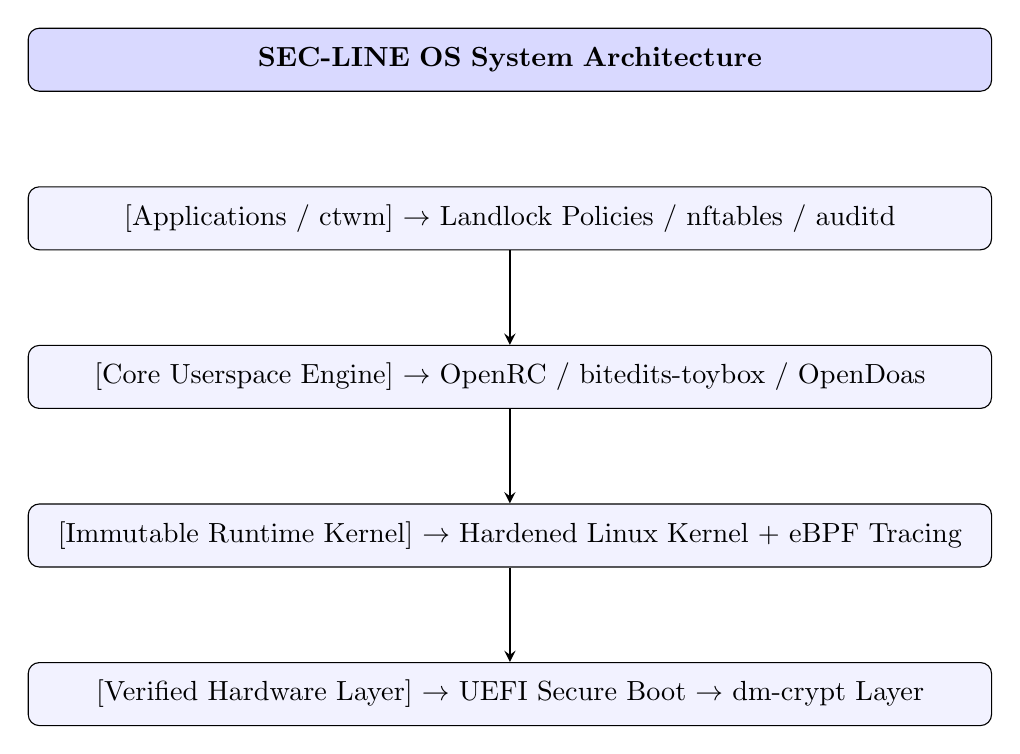
\begin{tikzpicture}[
    node distance=1.2cm,
    layer/.style={rectangle, draw, fill=blue!5, text width=12cm, text centered, minimum height=0.8cm, rounded corners},
    arrow/.style={thick, ->, >=stealth}
]
    \node (os) [layer, fill=blue!15] {\textbf{SEC-LINE OS System Architecture}};
    \node (apps) [layer, below=of os] {[Applications / ctwm] $\rightarrow$ Landlock Policies / nftables / auditd};
    \node (user) [layer, below=of apps] {[Core Userspace Engine] $\rightarrow$ OpenRC / bitedits-toybox / OpenDoas};
    \node (kern) [layer, below=of user] {[Immutable Runtime Kernel] $\rightarrow$ Hardened Linux Kernel + eBPF Tracing};
    \node (hw)   [layer, below=of kern] {[Verified Hardware Layer] $\rightarrow$ UEFI Secure Boot $\rightarrow$ dm-crypt Layer};

    \draw [arrow] (apps) -- (user);
    \draw [arrow] (user) -- (kern);
    \draw [arrow] (kern) -- (hw);
\end{tikzpicture}
\end{center}

\section{Architectural Pillars}
The design of SEC-LINE OS relies on four uncompromising principles:
\begin{itemize}
    \item \textbf{Cryptographic Immutability:} The entire base operating system kernel, configuration matrix, and initial execution files reside in a single, cryptographically signed binary.
    \item \textbf{Attack Surface Minimization:} Traditional distributions deploy up to several gigabytes of software. SEC-LINE OS strips the base rootfs down to its absolute mathematical minimum via custom forks (\texttt{bitedits/*}).
    \item \textbf{Process Isolation by Default:} Applications lack system-wide visibility. Access to the filesystem, network socket layers, and hardware inputs must be explicitly granted via declarative kernel policies.
    \item \textbf{State Separation:} The operating system treats runtime state as volatile. Persistent changes are restricted to dedicated, encrypted data blocks.
\end{itemize}

\section{The Secure Boot \& Storage Cryptography Pipeline}
SEC-LINE OS completely eliminates secondary bootloaders (e.g., GRUB, systemd-boot), which represent significant structural targets for Evil Maid attacks and persistent firmware exploitation.

\begin{center}
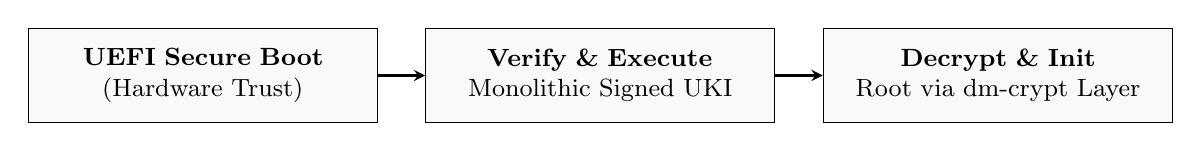
\begin{tikzpicture}[
    node distance=0.6cm,
    stepbox/.style={rectangle, draw, fill=gray!5, text width=4.2cm, text centered, minimum height=1.2cm, font=\small},
    arrow/.style={thick, ->, >=stealth}
]
    \node (uefi) [stepbox] {\textbf{UEFI Secure Boot}\\(Hardware Trust)};
    \node (uki)  [stepbox, right=of uefi] {\textbf{Verify \& Execute}\\Monolithic Signed UKI};
    \node (crypt)[stepbox, right=of uki] {\textbf{Decrypt \& Init}\\Root via dm-crypt Layer};

    \draw [arrow] (uefi) -- (uki);
    \draw [arrow] (uki) -- (crypt);
\end{tikzpicture}
\end{center}

\subsection{Unified Kernel Image (UKI) Construction}
The system builds a monolithic \texttt{zencrypted-os.efi} file containing:
\begin{enumerate}
    \item An official UEFI boot stub (\texttt{systemd-stub} stripped of systemd execution logic).
    \item A highly tailored, hardened Linux kernel.
    \item The system kernel command line (hardcoded at compile-time to prevent boot parameter injection).
    \item A minimal, specialized stage-1 \texttt{initramfs}.
\end{enumerate}

\subsection{Cryptographic Verification}
During machine activation, the hardware firmware evaluates the UKI against custom Platform Keys (\texttt{PK}/\texttt{KEK}/\texttt{db}) enrolled in the motherboard NVRAM. If verification succeeds, control hands off directly to the kernel execution thread.

\subsection{Early-Stage Disk Decryption (\texttt{dm-crypt})}
The immutable \texttt{initramfs} instantiates a minimal storage driver stack to invoke Linux kernel cryptography routines.
\begin{itemize}
    \item The primary system partition is validated and decrypted using \texttt{cryptsetup} with \texttt{dm-crypt} (AES-XTS-PLAIN64).
    \item Storage headers are detached or randomized to obscure partition bounds.
    \item Once authentication passes, the root filesystem mounts as a read-only device, executing a \texttt{switch\_root} loop into the main operating workspace.
\end{itemize}

\section{Kernel Architecture \& Security Profiles}
The operating system runs an optimized downstream derivation of the Linux Hardened kernel, prioritizing compile-time exploit mitigation over raw benchmark optimizations.

\subsection{Core Hardening Flags}
The kernel configuration enforces:
\begin{itemize}
    \item Strict Page Table Isolation (\texttt{PAGE\_\allowbreak TABLE\_\allowbreak ISOLATION=y}).
    \item Kernel Stack Randomization on system calls (\texttt{RANDOMIZE\_\allowbreak KSTACK\_\allowbreak OFFSET=y}).
    \item Complete memory wiping on allocation/deallocation boundary conditions (\texttt{INIT\_\allowbreak ON\_\allowbreak ALLOC\_\allowbreak DEFAULT\_\allowbreak ON=y}).
\end{itemize}

\subsection{Mandatory Access Control via Landlock LSM}
Unlike legacy MAC systems (SELinux/AppArmor) which add complex policy layers and complex tooling, SEC-LINE OS implements process sandboxing via \textbf{Landlock}.
\begin{itemize}
    \item \textbf{Mechanism:} Utilizing unprivileged sandboxing features, processes restrict their own filesystem actions and access paths.
    \item \textbf{Configuration:} The userspace engine utilizes \texttt{landlockconfig} to ingest declarative TOML rule structures at application initialization.
\end{itemize}

\begin{Verbatim}[frame=single, label=Example System Profile: /etc/landlock/ctwm.toml, breaklines=true, fontsize=\small]
[sandbox]
handled_access_fs = ["execute", "read_file", "read_dir", "write_file"]

[[rules.fs]]
path = "/usr/bin/ctwm"
access = ["execute", "read_file"]

[[rules.fs]]
path = "/home/zencrypted/.ctwmrc"
access = ["read_file"]
\end{Verbatim}

\subsection{High-Fidelity Tracing \& Auditing (eBPF \& auditd)}
System behavior analysis relies on non-invasive inspection loops rather than intrusive hooking infrastructures.
\begin{itemize}
    \item \textbf{Auditing:} System call profiling is verified by \texttt{bitedits/audit-userspace}, capturing unauthorized privilege transition vectors and immediate file write signals.
    \item \textbf{eBPF Observability:} Leveraging \texttt{bpftrace} patched directly for \texttt{musl-libc} interfaces, security daemons monitor kernel tracepoints dynamically without requiring run-time structural alterations.
\end{itemize}

\section{Userspace Composition \& Fork Strategy}
SEC-LINE OS avoids standard GNU utils and \texttt{busybox} monoliths, selecting modular components customized and maintained under the \texttt{bitedits} repository tree.

\begin{center}
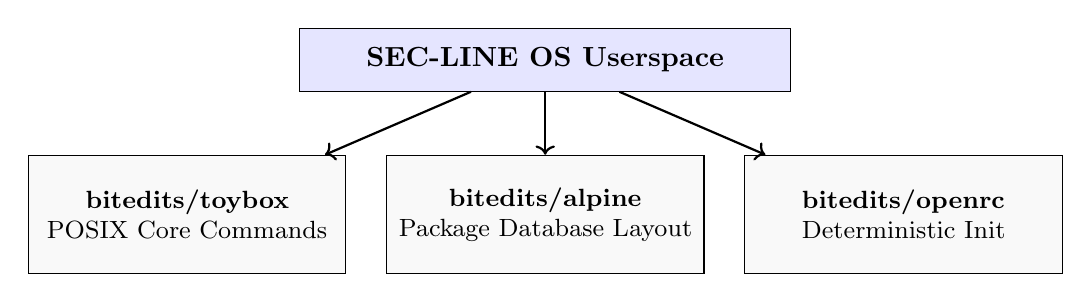
\begin{tikzpicture}[
    node distance=0.5cm,
    box/.style={rectangle, draw, fill=gray!5, text width=3.8cm, text centered, minimum height=1.5cm, font=\small},
    root/.style={rectangle, draw, fill=blue!10, text width=6cm, text centered, minimum height=0.8cm, font=\bfseries}
]
    \node (top) [root] {SEC-LINE OS Userspace};
    \node (mid) [box, below=of top, yshift=-0.3cm] {\textbf{bitedits/alpine}\\Package Database Layout};
    \node (left) [box, left=of mid] {\textbf{bitedits/toybox}\\POSIX Core Commands};
    \node (right) [box, right=of mid] {\textbf{bitedits/openrc}\\Deterministic Init};

    \draw [thick, ->] (top) -- (left);
    \draw [thick, ->] (top) -- (mid);
    \draw [thick, ->] (top) -- (right);
\end{tikzpicture}
\end{center}

\subsection{POSIX Engine: \texttt{bitedits/toybox}}
All vital system tools (\texttt{ls}, \texttt{ps}, \texttt{cat}, \texttt{chmod}) are provided via Rob Landley’s \texttt{toybox}. This deployment yields:
\begin{itemize}
    \item A clean breakpoint separating the system from bloated GNU software dependencies.
    \item Strict compliance with POSIX runtime directives.
    \item Symmetrical performance enhancements when interacting with memory operations over the \texttt{musl} API.
\end{itemize}

\subsection{Service Supervision: \texttt{bitedits/openrc}}
Process initialization follows a deterministic dependency graph managed by \texttt{openrc}.
\begin{itemize}
    \item \textbf{No Parallel Background Bloat:} Service dependencies map cleanly during build orchestration.
    \item \textbf{Predictable Execution Blocks:} Services run as unprivileged isolations where feasible, logging securely to stateless \texttt{/dev/log} pipes audited by \texttt{auditd}.
\end{itemize}

\subsection{Privilege Escalation: OpenDoas}
For administrative access loops, standard \texttt{sudo} is banned.
The system relies on \texttt{bitedits/OpenDoas}, enforcing:

\begin{itemize}
\item A code footprint less than 5\% of legavcy \texttt{sudo}.
\item Zero context persistence between separate shell instances.
\item Strict execution constraints mapped explicitly per user profile.
\end{itemize}

\section{Networking, Peripheral \& Graphical Environments}

The user interaction domain operates with the same minimal privileges as the core data routing architecture.

\subsection{Network Security Layer (\texttt{nftables})}

The firewall stack loads directly within the kernel image definition, adopting a strict \textbf{Default-Drop}
posture across all interface hooks:

\begin{Verbatim}[frame=single, label=nftables Core Configurations, breaklines=true, fontsize=\small]
table inet filter {chain input {type filter hook input priority filter;
policy drop;ct state established,related acceptiif "lo" accept}chain forward {type filter hook forward
priority filter; policy drop;}chain output {type filter hook output priority filter; policy drop;
udp dport 123 accept # Allowed: chrony NTP Synctcp dport 443 accept # Allowed: Outbound Encrypted TLS}}
\end{Verbatim}

\subsection{Seat and Input Management (\texttt{seatd})}

To operate a graphical workspace without a resource-heavy or complex display manager,
SEC-LINE OS links input routing through \texttt{seatd}.

\begin{itemize}
\item Grants application engines access to shared hardware
      interfaces (such as graphics cards or inputs) without
      requiring elevated \texttt{root} permissions.
\item Avoids any dependency on large user tracking packages,
      maintaining a tiny security perimeter for input tracking.
\end{itemize}

\subsection{Graphical Topography (\texttt{ctwm})}

The desktop layout is anchored by \texttt{ctwm} (Claude's Tab Window Manager).

\begin{itemize}
\item \textbf{Efficiency:} It runs inside an extremely lightweight system profile,
   bypassing modern desktop notification loops and complex message broker backplanes.
\item \textbf{Security:} Minimizes the visual display and rendering attack surface
   against local interface sniffing vectors.
\end{itemize}

\section{Package Lifecycle \& Supply Chain Integrity}

Software supply chains represent a primary target for sophisticated adversaries.
SEC-LINE OS maintains integrity through a strict binary deployment loop.

\begin{center}
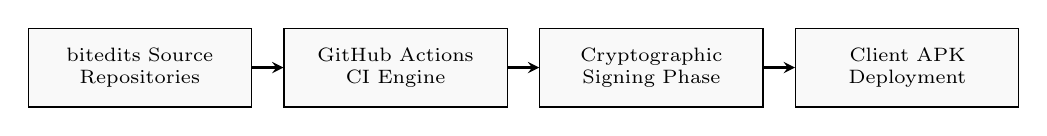
\begin{tikzpicture}[node distance=0.4cm,node/.style={rectangle, draw, fill=gray!5, text width=2.6cm,
     text centered, minimum height=1cm, font=\scriptsize},arrow/.style={thick, ->, >=stealth}]
     \node (src) [node] {bitedits Source\\Repositories};\node (ci)  [node, right=of src] {GitHub Actions\\CI Engine};
     \node (sign)[node, right=of ci] {Cryptographic\\Signing Phase};\node (apk) [node, right=of sign] {Client APK\\Deployment};
     \draw [arrow] (src) -- (ci);\draw [arrow] (ci) -- (sign);\draw [arrow] (sign) -- (apk);
\end{tikzpicture}
\end{center}

\begin{enumerate}
\item \textbf{Isolated Source Compilation:} Custom \texttt{APKBUILD} files fetch package source trees directly from validated \texttt{bitedits/*} endpoints.
\item \textbf{Deterministic Compilation:} Packages compile within automated, isolated pipelines generating reproducible hash check validations.
\item \textbf{Cryptographic Asset Signing:} Package outputs are packaged using Alpine's native Package Keeper (\texttt{apk-tools}) format and
      signed with an offline master key pair.
\item \textbf{Local Repository Integration:} The rootfs image builder installs signed \texttt{.apk}
      payloads directly into the OS structure, refusing any package lacking verified, local cryptographic signatures.
\end{enumerate}

\newpage
\section{Comparative Matrix}

\begin{table}[htbp]\centering\caption{System Parameter Architectural Baseline}
\label{tab:comparative_matrix}
\noindent\makebox[\textwidth][c]{
\begin{tabular}{p{4.2cm} p{7cm} p{7cm}}
\toprule\textbf{Security Parameter} & \textbf{Standard Enterprise Linux} & \textbf{SEC-LINE OS} \\
\midrule\textbf{Boot Mechanism} & UEFI $\rightarrow$ GRUB $\rightarrow$ Kernel $\rightarrow$ Initramfs & UEFI $\rightarrow$ Signed Monolithic UKI \\
\addlinespace\textbf{Boot Surface Tampering} & Vulnerable (Unsigned configs/modules) & Impossible (Breaks Secure Boot Signature) \\
\addlinespace\textbf{Core Utilities} & GNU Coreutils ($\sim$150MB, Complex) & \texttt{bitedits/toybox} ($<$5MB, Minimalist) \\
\addlinespace\textbf{Init Framework} & Complex asynchronous initialization & Monolithic, simple OpenRC system \\
\addlinespace\textbf{Default Sandbox Engine} & Process-wide (SELinux/AppArmor) & Thread-level declarative Landlock \\
\addlinespace\textbf{Privilege Transition} & Legacy Sudo Engine (Highly complex) & OpenDoas Framework (Audited, Minimal) \\
\bottomrule\end{tabular}
}\end{table}

\section{Conclusion}

SEC-LINE OS proves that modern hardware systems can be decoupled from complex, legacy distribution frameworks.
By consolidating the runtime layer inside an immutable Unified Kernel Image and enforcing strict sandboxing
across minimal userspace forks, SEC-LINE OS delivers an uncompromised, zero-trust infrastructure optimized
for high-assurance desktop layouts and isolated edge computation nodes.

\end{document}
